\documentclass[11pt,letterpaper]{article}

\usepackage[english]{babel}
\usepackage[utf8]{inputenc}

\usepackage{amsmath}
\usepackage{amssymb}
\usepackage{graphicx}

\usepackage[top=1in, bottom=1in, left=1in, right=1in]{geometry}
\graphicspath{{./imagenes/}} 

\begin{document}
	
	\begin{titlepage}
		\centering
		
		{\scshape\LARGE Universidad Nacional Autónoma de México \par}
		
		\vspace{1cm}
		{\scshape\Large Facultad de Ciencias\par}
		\vspace{1.5cm}
		
		\begin{figure}[h]
			\centering
			
\includegraphics[scale=0.15]{logo.png}
		\end{figure}
	
		\vspace{.8 cm}
		
		{\LARGE Práctica 01 \par}
		
		\vspace{0.5cm}
		\large{\itshape{Vianey Aileen Borrás Pablo}} \small{ - 316033619} \\ \vspace{0.3cm}
		\large{\itshape{Kevin Axel Prestegui Ramos}} \small{ - 316201373} \\ \vspace{0.3cm}
		\vfill
		
		\textbf{Arquitectura de Computadoras}\\
		\textbf{Dr. Jorge Luis Ortega Arjona}. \par
		\vspace{0.5cm}
		Fecha de entrega: \textbf{03 de marzo de 2020}.
	\end{titlepage}
 
\textbf{REPORTE PRÁCTICA 01}
\begin{itemize}
	
	\item \textbf{Circuito 1}\\
	Para hacer este circuito, se usó un AND y tres NOT, ya que no podíamos ocupar directamente la compuerta OR, así que lo primero que hicmos fue hacer la tabla de verdad del OR y después hacer la tabla de su equivalencia, en dicha tabla se puede observar que para obtener OR se necesita negar "x" y "y" y después negar toda la formula.
	\begin{itemize}
		\item \textbf{Ejemplo:}\\
		$\cdot$ 1 $\lor$ 1 = 1 \\
		$\cdot$ $\neg$ ($\neg$1 $\land$ $\neg$ 1) = $\neg$ (0 $\land$ 0) = 1 $\lor$ 1 =1		
	\end{itemize}
		
		\begin{figure}[h]
			\centering
			
\includegraphics[scale=0.15]{TOR.png}\\
			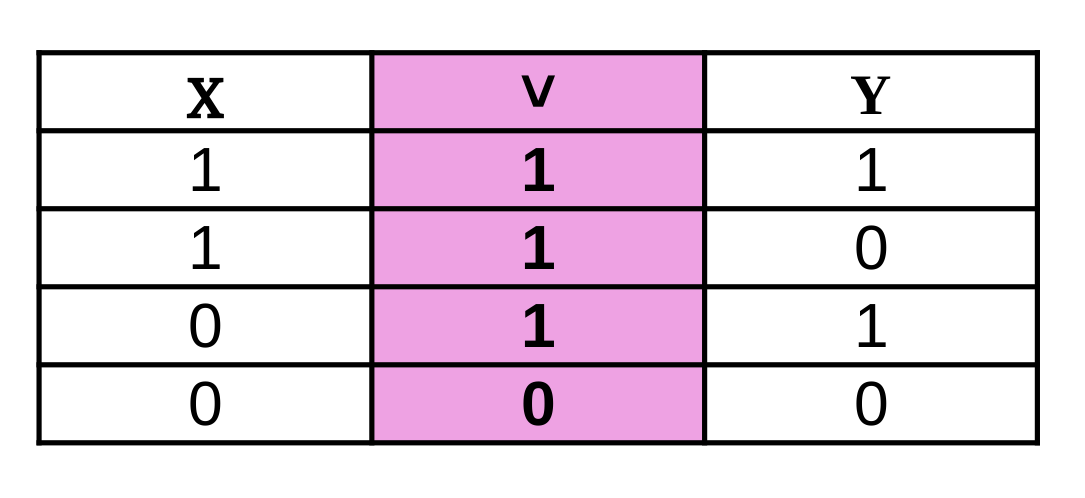
\includegraphics[scale=0.15]{OR.png}
			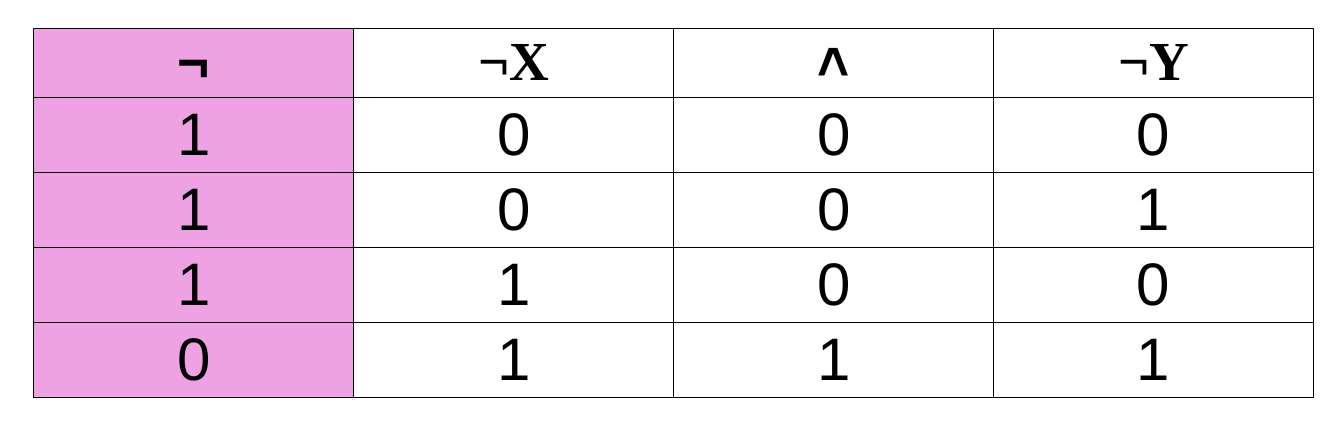
\includegraphics[scale=0.15]{EquivalenciaOR.png}
			\caption{OR y su equivalencia}
		\end{figure}
	
	Una vez terminada ambas tablas, construimos el circuito a partir de las tablas de verdad, específicamente la de la equivalencia. En la imágen se observa que utilizamos dos NOT como entrada, después un AND y finalmente otro NOT que es la interpretación de nuestra tabla de verdad (equivalencia de OR).
	
	\begin{figure}[h]
		\centering
		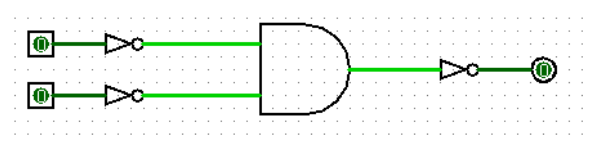
\includegraphics[scale=0.5]{CircuitoOR.png}
		\caption{Circuito OR, sin usar la compuerta OR}
	\end{figure}


	Probando la tabla de verdad en el circuito, observemos que en efecto funciona, donde si la entrada/salida esta encendida es 1 en otro caso es 0.
	
	\begin{figure}[h]
		\centering
		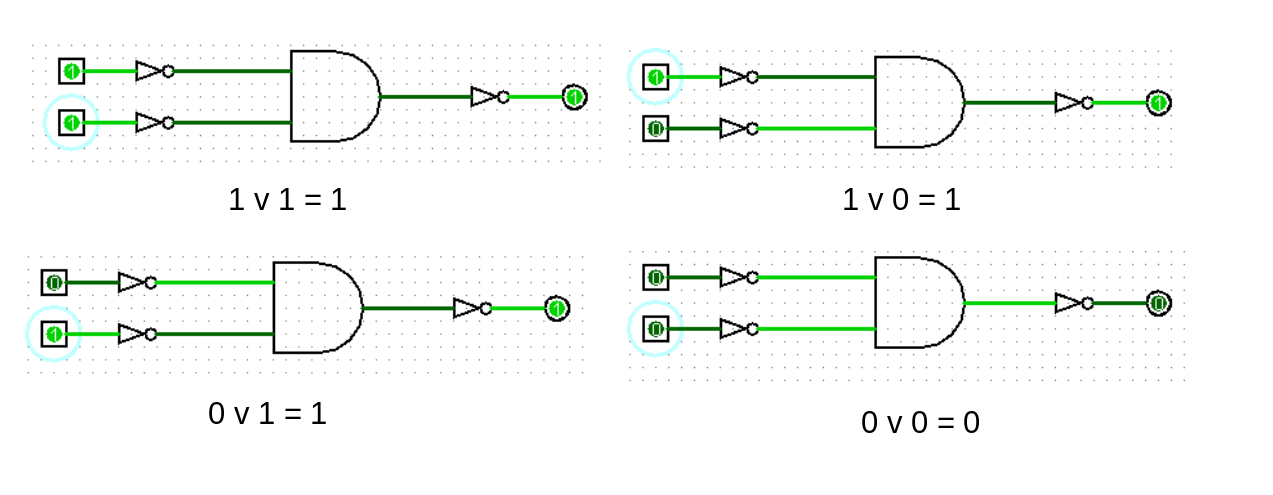
\includegraphics[scale=0.24]{CircOR.png}
		\caption{Circuito OR con distintos valores }
	\end{figure}
			


	\item \textbf{Circuito 2}\\
	
	Ahora se pidió que se realizaran dos circuitos uno que simule el comportamiento de la implicación lógica ($\rightarrow$) y otro que es su equivalencia. Para poder hacer los circuitos lo primero que hicimos fue realizar la tabla de verdad de la implicación, con base a la tabla de verdad pudimos hacer las tablas de verdad que simula la implicación y su equivalencia.
		
		\begin{figure}[h]
			\centering
			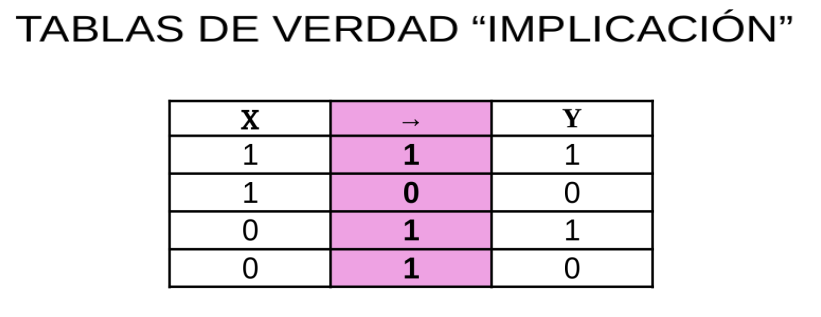
\includegraphics[scale=0.35]{Imp.png}
			\caption{Tabla de verdad de la implicación}			
		\end{figure}
	
		\begin{figure}[h]
			\centering
			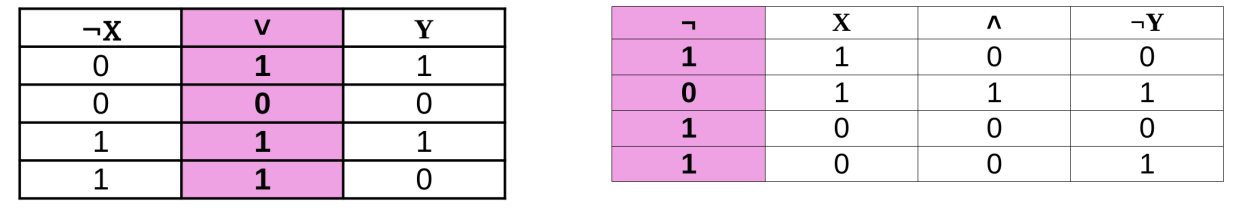
\includegraphics[scale=0.35]{Impyequivalencia.png}
			\caption{Simulación de la implicación y su equivalencia}
		\end{figure}
	
	Observemos que para poder construir un circuito que simula la implicación se necesita negar a "x" aplicar OR y los valores de "y" se quedan igual, y para obtener su equivalencia dejamos los valor de "x" igual, aplicamos AND, negamos los valores de "y" y finalmente negamos todo.
	
	\begin{itemize}
		\item \textbf{Ejemplo:}\\
		$\cdot$ 1 $\rightarrow$ 1 = 1\\
		$\cdot$ $\neg$1 $\lor$ 1 = 0 $\lor$ 1 = 1\\
		$\cdot$ $\neg$(1 $\land$ $\neg$1) = $\neg$(1 $\land$ 0) = $\neg$(0) = 1
	\end{itemize}
	
	\begin{figure}[h]
		\centering
		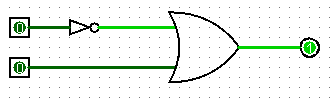
\includegraphics[scale=0.55]{Implicacion.png}
		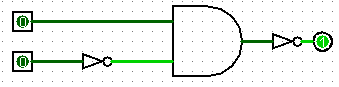
\includegraphics[scale=0.55]{EquivImp.png}
		\caption{circ. que simula la implicaión, y su equivalencia}
	\end{figure}
	
	$\\$
	\\
	
	Si probamos la tabla de verdad de la implicación en ambos circuitos observamos que en efecto funcionan.
	
	\begin{figure}[h]
		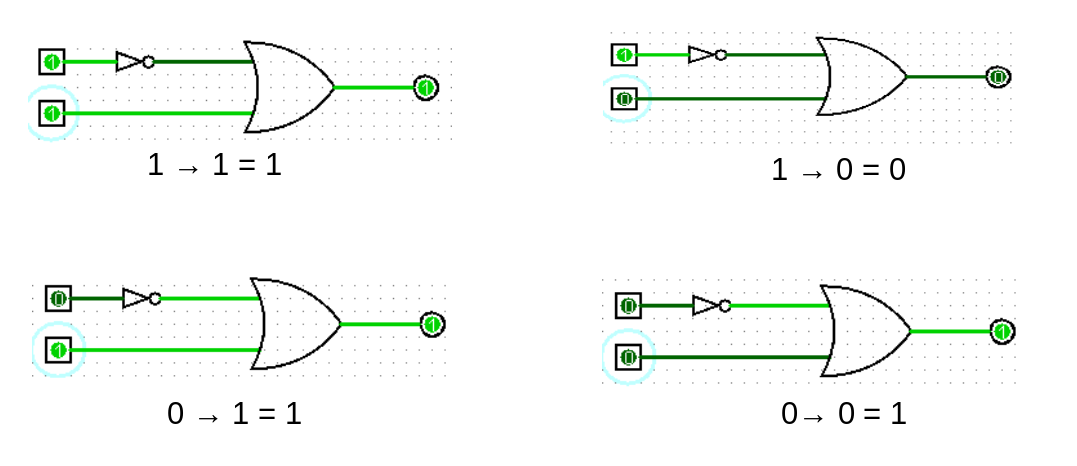
\includegraphics[scale=0.24]{PruebaImp.png}
		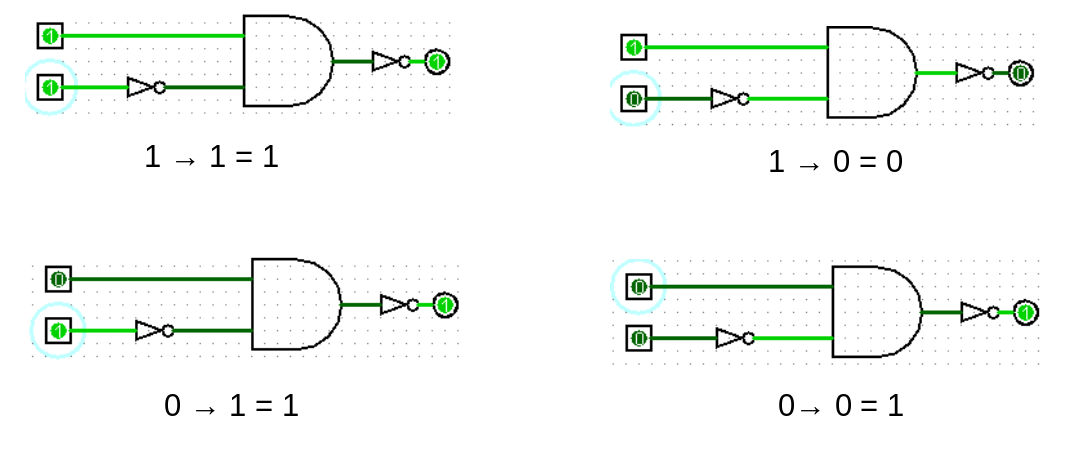
\includegraphics[scale=0.24]{PruebaImpEquiv.png}
		\caption{Circuitos con distintos valores}
	\end{figure}

	\item \textbf{Circuito 3}\\
	
	Se pide que se realicen dos circuitos uno que simule el comportamiento de la doble implicación lógica ($\leftrightarrow$) y otro que es su equivalencia. Para poder hacer los circuitos se hizo lo mismo que en el circuito anterior(construir las tablas de verdad).
	
	\begin{figure}[h]
		\centering
		
\includegraphics[scale=0.5]{TDI.png}
		
		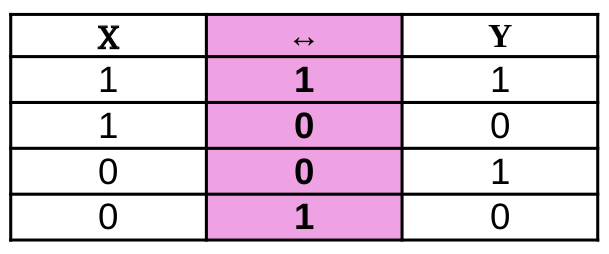
\includegraphics[scale=0.30]{DI.png}
		\caption{Tabla de verdad de la doble implicación}
		
		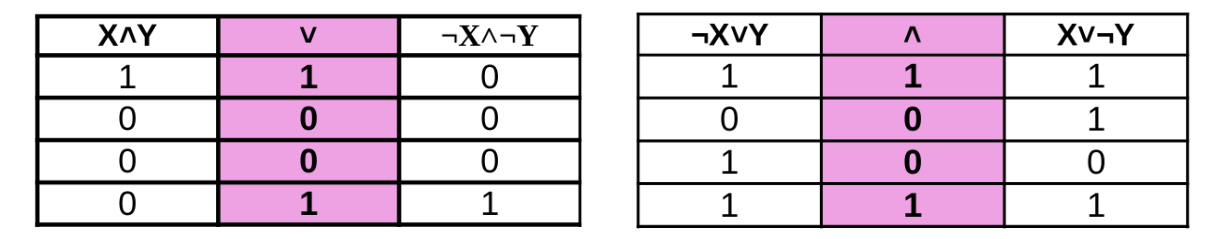
\includegraphics[scale=0.40]{DIyE.png}
		\caption{Simulación de la doble implicación y su equivalencia}
	\end{figure}

	Con la primera tabla de la figura 9, podemos construir el circuito que simula la doble implicación y para poder construir un circuito equivalente se uso la segunda tabla de la figura 9 donde hicimos uso de la implicación.
	
	\begin{itemize}
		\item \textbf{Ejemplo:}\\
		$\cdot$ 1 $\leftrightarrow$ 1 = 1\\
		$\cdot$ (1 $\land$ 1) $\lor$ ($\neg$1 $\land$ $\neg$1) = (1) $\lor$ (0 $\land$ 0) = 1 $\lor$ 0 = 1\\
		$\cdot$ ($\neg$(1 $\lor$ 1) $\land$ (1 $\lor$ $\neg$1)) = (0 $\lor$ 1) $\land$ (1 $\lor$ 0) = 1 $\land$ 1 = 1
	\end{itemize}

	\begin{figure}[h]
		\centering
		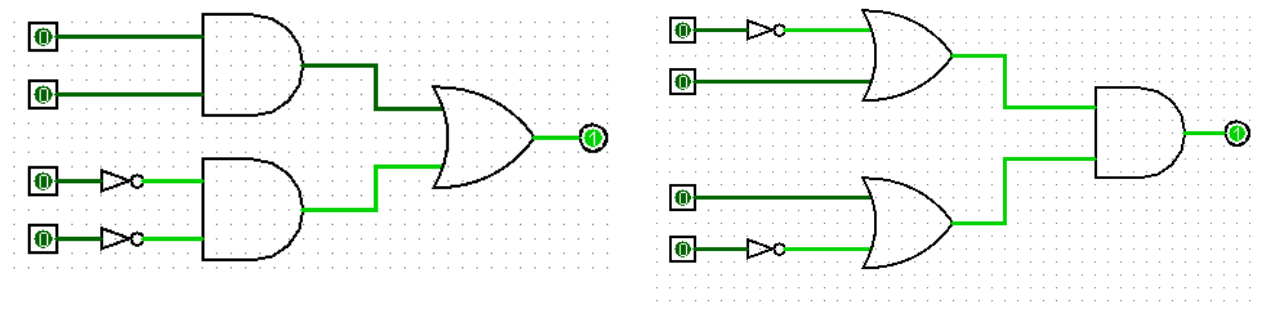
\includegraphics[scale=0.40]{CircDI.png}
		\caption{Circ. que simula la doble implicación y su equivalencia}
	\end{figure}
	
	Probando la tabla de verdad de la doble implicación en ambos circuitos observemos que funcionan.
	
	\begin{figure}[h]
		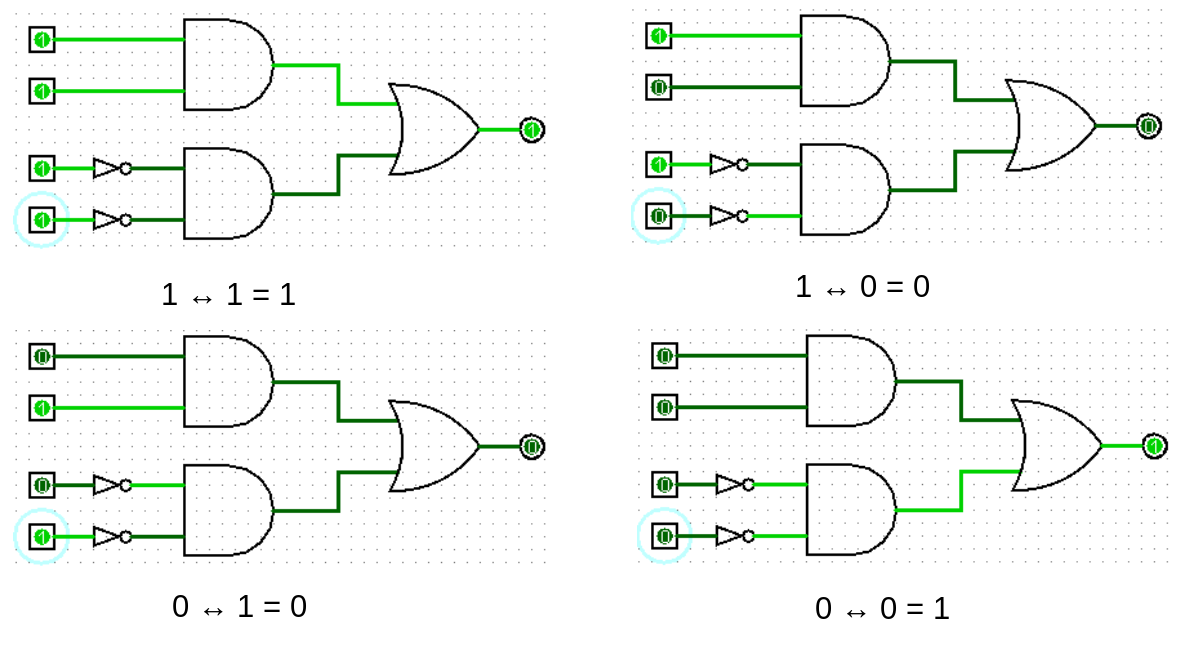
\includegraphics[scale=0.20]{PDI.png}
		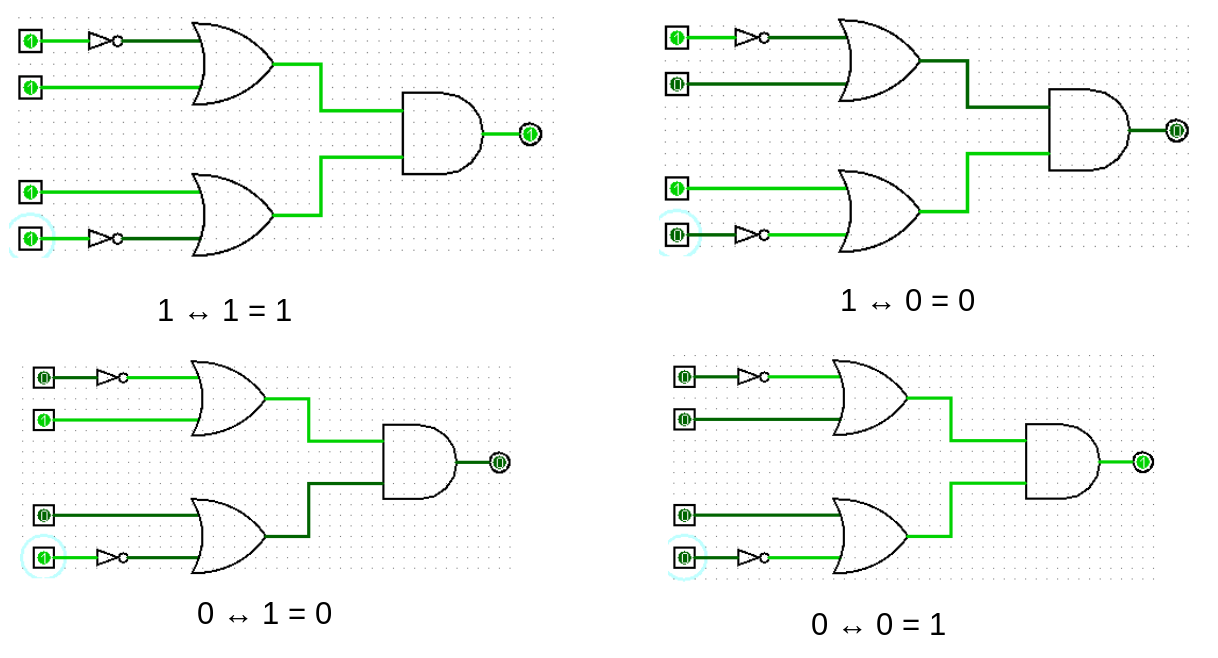
\includegraphics[scale=0.20]{PDIE.png}
		\caption{Circuitos con distintos valores}
	\end{figure}
	 
	 \newpage
	
	\item \textbf{Circuito 4}\\
	
	Para poder hacer el mecanismo de votación lo primero que hicimos fue hacer la tabla de verdad, para poder ver los casos en el que el led se enciende, este se va encender cuando haya exactamente 3 votos o más de lo contrario se quedara apagado, tomando en cuenta que 3 integrantes tienen derecho a un voto mientras que el voto de Tobi cuenta doble vez.
	
	\begin{figure}[h]
		\centering
		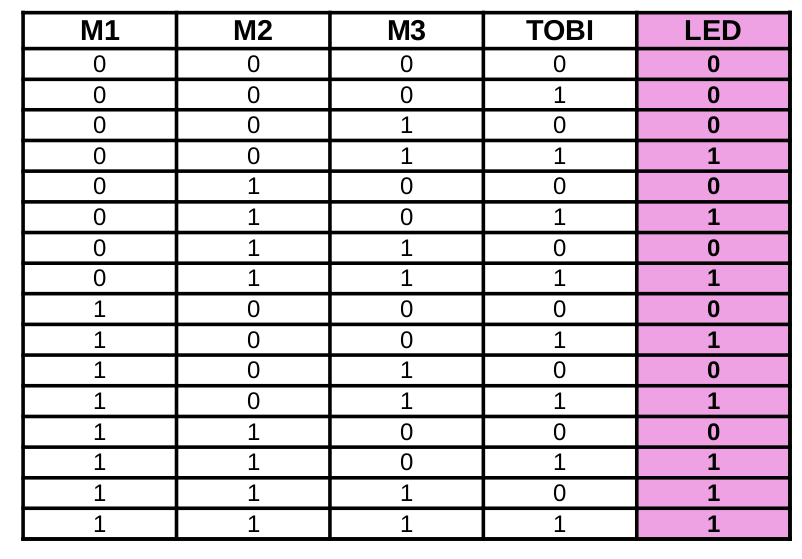
\includegraphics[scale=0.26]{TablaVot.png}
		\caption{Tabla de Verdad del LED}
	\end{figure}

	La fórmula para cuando el LED esta encendido con base a la tabla de verdad es:\\

	\textbf{LED encendido=} $\overline{a}$$\overline{b}$cd + $\overline{a}$b$\overline{c}$d + $\overline{a}$bcd + a$\overline{b}$$\overline{c}$d + a$\overline{b}$cd + ab$\overline{c}$d + abc$\overline{d}$ + abcd\\
	
	Así como esta la fórmula nos quedaría un circuito muy grande, por lo que decidimos minimizar la formula usando el mapa de Karnaugh.
	
	\begin{figure}[h]
		\centering
		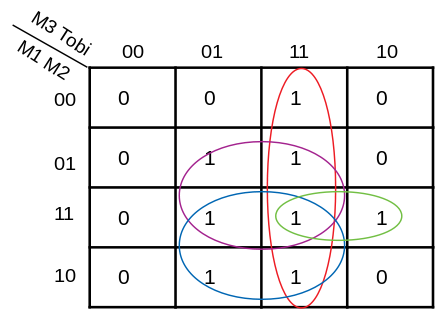
\includegraphics[scale=0.5]{Karnaugh.png}
		\caption{Mapa de Karnaugh}
	\end{figure}
	
	Ahora nuestra formula minimizada es \textbf{LED Encendido=} ad + bd + cd + abc\\
	Donde: a = M1\\
	\hspace*{1.3cm} b = M2\\
	\hspace*{1.3cm} c = M3\\
	\hspace*{1.3cm} d = Tobi
	
	Una vez que obtuvimos la formula minimizada procedimos a construir el circuito, observemos que en la fórmula hay multiplicación y sumas, por lo que usamos las compuertas AND y OR.
	
	\begin{figure}[h]
		\centering
		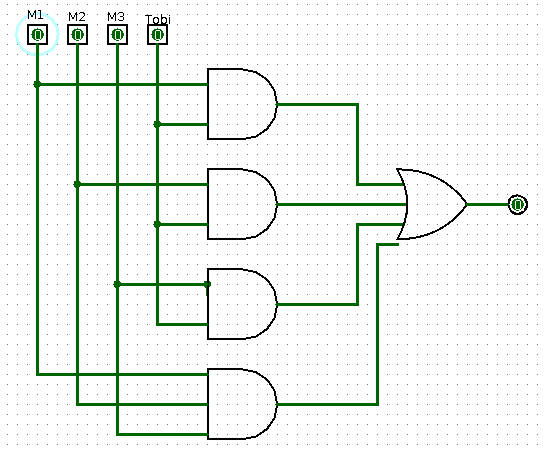
\includegraphics[scale=0.5]{CircVot.png}
		\caption{Circuito de un mecanismo de votación}
	\end{figure}

	Si probamos algunos valores de la tabla observemos que nuestro circuito funciona.
	
	\begin{figure}[h]
		\centering
		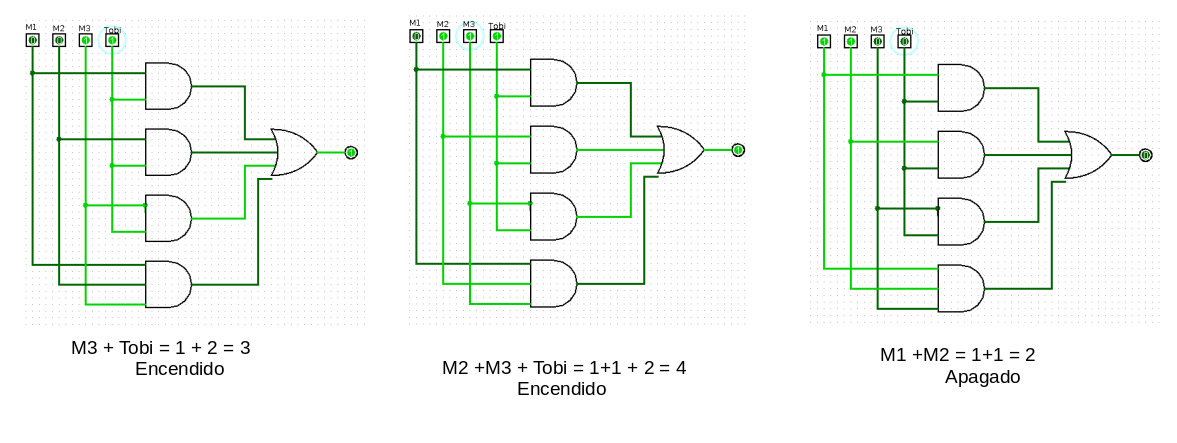
\includegraphics[scale=0.45]{Votaciones.png}
		\caption{Circuito de votación con algunos valores}
	\end{figure}
	
\end{itemize}

\end{document}